\documentclass[tikz]{standalone}

\usepackage{tikz}
\usetikzlibrary{positioning}
\usetikzlibrary{shadows}
\usetikzlibrary{shapes.arrows}

\usepackage{fontspec}

\setmainfont{TUOS Stephenson}
\setsansfont{TUOS Blake}
\renewcommand{\familydefault}{\sfdefault}

\begin{document}
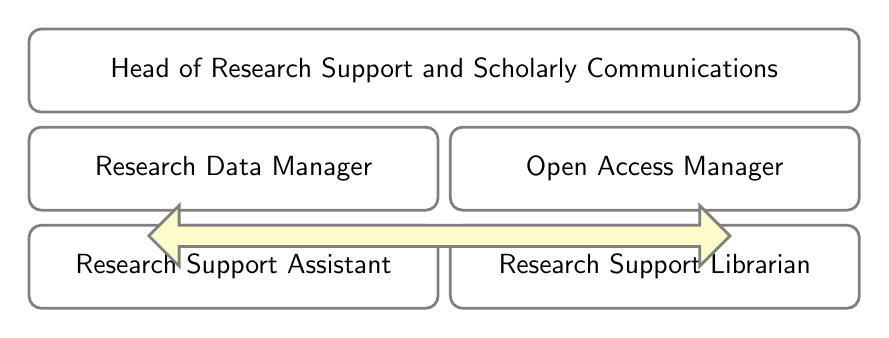
\begin{tikzpicture}[every node/.style={draw=black!50, fill=white, minimum height=3em, rounded corners=1ex, line width=1pt}]
  \node[minimum width=30em] (head) {Head of Research Support and Scholarly Communications};
  \begin{scope}[minimum width=15em-0.5ex]
    \node[below=1ex of head.south west,anchor=north west] (rdm)
      {Research Data Manager};
    \node[below=1ex of head.south east,anchor=north east] (oam)
      {Open Access Manager};
    \node[below=1ex of rdm] (rsa)
      {Research Support Assistant};
    \node[below=1ex of oam] (rsl)
      {Research Support Librarian};
    \node[shape=double arrow,%
      minimum width=0.5em, minimum height=21em,%
      fill=yellow!20, rounded corners=0,%
      below=1ex of rdm.south east] {};
  \end{scope}
\end{tikzpicture}
\end{document}
